\documentclass[usepdftitle=false,hyperref={pdfpagelabels=false}]{beamer}

% use KIT-Theme
% see http://sdqweb.ipd.kit.edu/wiki/Dokumentvorlagen
%\usetheme{Frankfurt} % see http://deic.uab.es/~iblanes/beamer_gallery/index_by_theme.html as fallback
\InputIfFileExists{../templates/beamerthemekit.sty}{\usepackage{../templates/beamerthemekit}}{\usetheme{Frankfurt}}
\usefonttheme{professionalfonts}

\usepackage{hyperref}
\usepackage{lmodern}
\usepackage{listings}
\usepackage{wrapfig}        % see http://en.wikibooks.org/wiki/LaTeX/Floats,_Figures_and_Captions
\usepackage[utf8]{inputenc} % this is needed for german umlauts
\usepackage[ngerman]{babel} % this is needed for german umlauts
\usepackage[T1]{fontenc}    % this is needed for correct output of umlauts in pdf
\usepackage{verbatim}
\usepackage{relsize}
\usepackage{subfigure}
\usepackage{algorithm,algpseudocode}
\usepackage{minted}         % needed for the inclusion of source code
\usepackage{menukeys}
\usepackage{xcolor}
\usepackage{pifont}% http://ctan.org/pkg/pifont
\newcommand{\cmark}{\ding{51}}%
\newcommand{\xmark}{\ding{55}}%
\usepackage{../templates/myStyle}

\newcommand\tutor{Martin Thoma}
\newcommand\tutNR{10}
\newcommand\titleText{Programmieren-Tutorium Nr. \tutNR{} bei \tutor}
\institute{Fakultät für Informatik}

\hypersetup{pdftitle={\titleText}}
\beamertemplatenavigationsymbolsempty

\newcommand\InsertToC[1][]{
  \begin{frame}{Outline}
    \tableofcontents[subsectionstyle=show/show/show, subsubsectionstyle=show/show/show, #1]
  \end{frame}
}

\begin{document}
\title{\titleText}
\subtitle{Pakete}
\author{\tutor}
\date{\today}
\subject{Programmieren}

\frame{\titlepage}

\frame{
    \frametitle{Inhaltsverzeichnis}
    \setcounter{tocdepth}{1}
    \tableofcontents
    \setcounter{tocdepth}{2}
}

\section{Einleitung}
\subsection{Quiz}
\begin{frame}{Quiz}
    \begin{minipage}[b]{0.45\linewidth}
        \inputminted[linenos=false, numbersep=5pt, tabsize=4, fontsize=\tiny, label=String.java, frame=lines]{java}{String.java}
    \end{minipage}
    \hspace{0.5cm}
    \begin{minipage}[b]{0.45\linewidth}
        \inputminted[linenos=false, numbersep=5pt, tabsize=4, fontsize=\tiny, label=World.java, frame=lines]{java}{World.java}
    \end{minipage}
    \begin{itemize}
        \item Gibt es einen Compiler-Fehler?
        \item Gibt es einen Laufzeit-Fehler?
        \item Gibt es eine Ausgabe? Welche?
    \end{itemize}
\end{frame}

\begin{frame}{Ergebnis}
    \myCode{Exception in thread "main" java.lang.NoSuchMethodError: main}\\
    Es gibt nun keine \\
    \myCode{public static void main(java.lang.String[] args) \{}\\
    \begin{block}{Lehre}
        Keine Java-internen Typen umschreiben.
    \end{block}
\end{frame}


\section{ÜB 2}
\subsection{Nachbesprechung ÜB 2}
\begin{frame}{Allgmeines}
    \begin{block}{Musterlösung}
        Inoffizielle Musterlösung von Simon und mir ist unter
        \href{http://goo.gl/BfA6i}{http://goo.gl/BfA6i} erhältlich.\\
        Bitte dort anschauen.
    \end{block}
\end{frame}

\begin{frame}{Allgmeines}
  \begin{block}{Stil}
    \begin{itemize}[<+->]
        \item Niemals \myCode{if (variable == true)}, sondern \myCode{if (variable)}
        \item "`Dead Code"' - also Code der niemals erreicht wird - wird bestraft
        \item Große Probleme ($\rightarrow$ lange Methoden) aufsplitten
    \end{itemize}
  \end{block}

    \begin{itemize}[<+->]
        \item Die bereitgestellten Code-Vorlagen sind keine Musterlösungen!
        \item Kein "`TODO"' in Abgaben
        \item Aufgabe B1 (Histogramm) war fehlerhaft: Natürlich muss der Kontrast nur "`nicht-negativ"' sein und nicht "`positiv"'
        \item Laufvariablen müssen nicht immer \myCode{i} und \myCode{j} heißen
        \item Schaut euch die hochgeladeten Dateien im Praktomat an
        \item Redundanter Code ist schlecht $\Rightarrow$ Besser: Neue Methode anlegen
    \end{itemize}
\end{frame}

\begin{frame}{Allgemeines}
    \begin{block}{Genau lesen}
      \begin{itemize}[<+->]
        \item \textbf{A.1.1 Konstruktor von Bike}: "`Modifizieren Sie
              den Konstruktor der Klasse Bike, indem Sie aus der
              Signatur das Argument, nach dem bisher der Preis
              gesetzt wird, entfernen."'
        \item \textbf{A.1.2 Setter für Gears} "`Schreiben Sie den
              Konstruktor so um,  dass er die Methode setSprockets
              benutzt, um einen  konsistenten Anfangszustand zu
              garantieren."'
        \item \textbf{A.2.1 Tribonacci-Folge}: "`Geben Sie \textbf{nur} die
              siebenunddreißigste Tribonacci-Zahl auf der Konsole
              aus."'
        \item[$\Rightarrow$] Es werden automatische Tests durchgeführt.
              Stimmt die Ausgabe nicht exakt - also jedes einzelne
              (Leer)zeichen -, schlägt der Test fehl.
      \end{itemize}
    \end{block}
\end{frame}

\begin{frame}{Tipp für BikeShop}
   \myCode{\href{http://docs.oracle.com/javase/7/docs/api/java/lang/System.html\#arraycopy(java.lang.Object, int, java.lang.Object, int, int)}{System.arraycopy(warehouse, 0, newStock, 0, warehouse.length);}}
\end{frame}

\begin{frame}{setSprockets}
    \inputminted[linenos=false, numbersep=5pt, tabsize=4, fontsize=\tiny, label=Gears.java, frame=lines, firstline=25, lastline=51]{java}{Gears.java}
\end{frame}

\begin{frame}{Einheiten}
  Einheiten \textbf{immer} angeben, da \dots
  \begin{itemize}[<+->]
    \item nie klar ist, welche Einheit gemeint ist
    \item es ein richtig ärgerlicher Fehler ist
    \item fehlende Einheiten viel Geld kosten können ($\rightarrow$ \href{http://www.youtube.com/watch?v=q2L5\_swAT5A}{Video: NASA Measuring Failure} - Mars Orbiter)
  \end{itemize}
\end{frame}

\begin{frame}{Attribute}
  \begin{alertblock}{Attribute}
    \begin{itemize}
      \item Attribute sind Eigenschaften eines Objekts oder einer Klasse
      \item Attribute sind keine Hilfsvariablen
    \end{itemize}
  \end{alertblock}
\end{frame}

\begin{frame}{Vergleiche mit floats}
    Nicht jede Zahl kann als Gleitkomma-Zahl dargestellt werden:
    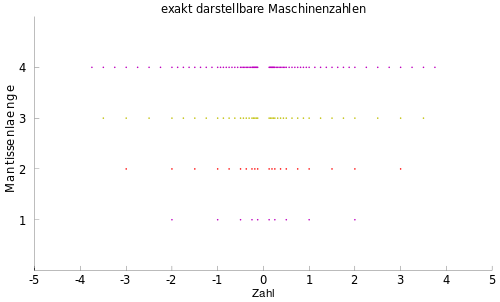
\includegraphics[height=50mm]{Gleitkommazahlen.png}\\
    \tiny{Quelle: \href{http://de.wikipedia.org/wiki/Datei:Gleitkommazahlen.svg}{de.wikipedia.org/wiki/Datei:Gleitkommazahlen.svg}}\\


\end{frame}

\begin{frame}{Vergleiche mit floats}
    Zusätzlich sollte man bei der Camera-Aufgabe von $\varepsilon = 10^6$ ausgehen.\\
    Die Vergleiche müssen also etwa so aussehen:
    \inputminted[linenos=false, numbersep=5pt, tabsize=4, fontsize=\small, firstnumber=24, firstline=24, lastline=33]{java}{Camera.java}
\end{frame}

\begin{frame}{Camera.java: isLeftContrastHigher}
    \inputminted[linenos=true, numbersep=5pt, tabsize=4, fontsize=\tiny, firstnumber=35, firstline=35, lastline=55]{java}{Camera.java}
\end{frame}

\begin{frame}{Camera.java: Eigentlicher Code}
    \inputminted[linenos=true, numbersep=5pt, tabsize=4, fontsize=\tiny, firstnumber=57, firstline=57, lastline=87]{java}{Camera.java}
\end{frame}

\begin{frame}{Gerüchteküche}
  Bringt es einen Vorteil, eine schwere Aufgabe nicht zu bearbeiten?
  \begin{itemize}[<+->]
    \item Es gibt für jede Teilaufgabe ein Punktekontingent
    \item Bearbeitet ihr eine Teilaufgabe nicht, ziehe ich alle Punkte ab
    \item Bearbeitet ihr einen Teil einer Teilaufgabe nicht, ziehe
          ich mindestens so viele Punkte ab, wie derjenige mit dem
          höchstem Abzug abgezogen bekommen hat
    \item Wenn der Code nicht das tut, was gefordert wird, kann ich
          auch alles abziehen
    \item[$\Rightarrow$] Nein, es bringt keinen Vorteil
  \end{itemize}
\end{frame}

\section{Vorlesungsergänzungen}
\subsection{Pakete}
\begin{frame}{Pakete}
    \begin{itemize}[<+->]
      \item Dienen der Strukturierung des Quelltextes
      \item Sollen Namenskonflikte vermeiden (z.B. Klasse \myCode{Person}
            in einem Paket \myCode{uni} ist wohl anders als Klasse
            \myCode{Person} im Paket \myCode{politik})
      \item Können über \myCode{.jar}-Dateien eingebunden werden
      \item Könnt ihr über \keys{\shift + Alt + N} und \menu{Package}
            oder mit einem Rechtsklick in Eclipse erzeugen:
        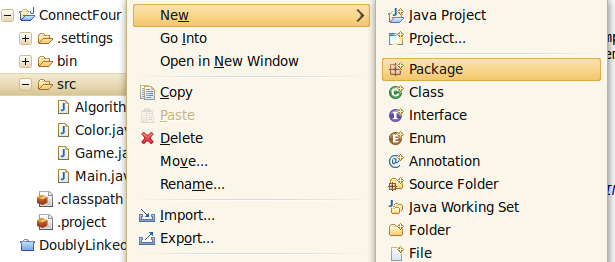
\includegraphics[height=30mm]{new-package.png}\\
      \item Eine Klasse ist Teil eines Paketes, wenn sie \dots
        \begin{itemize}
            \item in dem Ordner mit dem Paketnamen liegt
            \item sie \myCode{package <paketname>;} ganz am Anfang stehen hat
        \end{itemize}
    \end{itemize}
\end{frame}

\begin{frame}{Pakete}
    \begin{block}{Namenskonventionen}
        \begin{itemize}
            \item Pakete werden klein geschrieben
            \item Pakete können "`Unterpakete"' haben. Dies wird durch
                  einen Punkt angedeutet:
              \begin{itemize}
                \item \href{http://docs.oracle.com/javase/7/docs/api/overview-summary.html}{Offizielle Pakete}:
                \item \href{http://docs.oracle.com/javase/7/docs/api/java/io/package-summary.html}{java.io}
                \item \href{http://docs.oracle.com/javase/7/docs/api/java/lang/package-summary.html}{java.lang} - hat z.B. \myCode{Byte}, \myCode{Integer}, \dots
                \item \href{http://docs.oracle.com/javase/7/docs/api/java/lang/annotation/package-summary.html}{java.lang.annotation}
              \end{itemize}
        \end{itemize}
    \end{block}
\end{frame}

\begin{frame}{Pakete: protected}
    \begin{tabular}{l||c|c|c|c}
        Modifier            & Class & Package   & Subclass  & World\\
        \hline\hline
        \myCode{public}     & \cmark & \cmark & \cmark & \cmark \\
        \myCode{protected}  & \cmark & \cmark & \cmark & \xmark \\
        no modifier         & \cmark & \cmark & \xmark & \xmark \\
        \myCode{private}    & \cmark & \xmark & \xmark & \xmark
    \end{tabular}

    \small{Weitere Informationen: \href{http://docs.oracle.com/javase/tutorial/java/javaOO/accesscontrol.html}{Controlling Access to Members of a Class}}
    \pause
    \begin{block}{Tipp}
        \myCode{private} macht fast immer Sinn. Wenn ihr nicht wisst,
        ob ihr \myCode{private} oder \myCode{protected} nehmen sollt,
        nehmt protected. Kein modifier macht selten Sinn. Das sieht
        so aus, als ob ihr es dem Zufall überlasst.
    \end{block}
\end{frame}

\subsection{foreach-Schleife}
\begin{frame}{foreach in Java: Allgemeines}
    Foreach \dots
    \begin{itemize}[<+->]
        \item wird in Java-Kreisen manchmal auch "`Enhanced for loop"' genannt
        \item geht alle Elemente einer
              \href{http://docs.oracle.com/javase/7/docs/api/java/util/Collection.html}{Collection}
              durch zu gehen (genauer: \href{http://docs.oracle.com/javase/7/docs/api/java/lang/Iterable.html}{Iterable})
        \item sollte verwendet werden, wenn man es verwenden kann
        \item ist auch in der \href{http://docs.oracle.com/javase/1.5.0/docs/guide/language/foreach.html}{Dokumentation} (Nur in 1.5?)
              und im \href{http://docs.oracle.com/javase/tutorial/java/nutsandbolts/for.html}{Tutorial}
        \item ist in der \href{http://docs.oracle.com/javase/specs/jls/se7/html/jls-14.html\#jls-14.14.2}{JLS SE7} spezifiziert
        \item ist Teil des \href{http://docs.oracle.com/javase/tutorial/extra/certification/javase-7-programmer1.html}{Programmer Level I Exams}
              für das "`Programmer Language Certification"'
    \end{itemize}
\end{frame}
\begin{frame}{foreach in Java: Beispiel}
    \inputminted[linenos=false, numbersep=5pt, tabsize=4, fontsize=\small, firstline=3, lastline=13]{java}{foreach.java}
\end{frame}

\section{ÜB 3}
\subsection{Hinweise zu ÜB 3}
\begin{frame}{Hinweise zu ÜB 3}
  \begin{itemize}[<+->]
    \item Nur Klassen und Methoden aus \myCode{java.lang} sind erlaubt
    \item \textbf{Keine} Textausgabe und keine Schreibzugriffe auf Dateien
    \item JavaDoc und Datenkapselung ($\rightarrow$ \myCode{private}) sind nun Pflicht
    \item Pakete sollten nun verwendet werden
    \item[$\Rightarrow$] Achtung beim Upload in den Praktomaten! vgl. tutorium-05.pdf, Folien 23-24
    \item[A.1.1] Nur die \myCode{statements.csv} als Abgabe!
    \item[A.2] \myCode{StrangeClass.java} soll wirklich \textbf{nirgends} "`f"' und kein "`d"' haben
    \item[A.3] Levenshtein-Distanz $\rightarrow$ nächste Folie
    \item[A.4] Geometrie $\rightarrow$ übernächste Folie
    \item[B.1] Der Kommentar, warum ihr die Modifier (\myCode{private, public, protected})
               verwendet, soll natürlich direkt zum jeweiligen modifier und NICHT in
               eine extra Textdatei!
  \end{itemize}
\end{frame}

\subsection{Levenshtein-Distanz}
\begin{frame}{A.3 Levenshtein-Distanz}
  \begin{itemize}[<+->]
    \item Wer hat sichs angeschaut?
    \item Verstanden? Falls nicht sind folgende Seiten einen Versuch wert:
    \begin{itemize}
        \item \href{http://oldfashionedsoftware.com/tag/levenshtein-distance/}{Guter Artikel}, aber nur bis "`Some Code, Finally"' relevant
        \item \href{http://de.wikipedia.org/wiki/Levenshtein-Distanz}{de-Wikipedia}
        \item \href{http://en.wikipedia.org/wiki/Levenshtein_Distance\#Computing_Levenshtein_distance}{en-Wiki} mit Pseudocode
        \item \href{http://www-igm.univ-mlv.fr/~lecroq/seqcomp/node2.html}{eine Visualisierung}
    \end{itemize}
    \begin{alertblock}{Achtung!}
      Der Algorithmus muss modifiziert werden. Durch die Modifikationen entspricht
      der Algorithmus nicht mehr den Varianten, die sich im Internet finden lassen.
      Ohne diese Modifikationen kann ich euch keine Punkte geben!
    \end{alertblock}
  \end{itemize}
\end{frame}

\subsection{A.4 Geometrie}
\begin{frame}{A.4 Geometrie}
  \begin{itemize}[<+->]
    \item Manhattan-Distanz:\\
        \includegraphics[height=30mm]{ManhattanDistance.pdf}\\
        \tiny{Quelle: \href{http://commons.wikimedia.org/wiki/File:Manhattan\_distance.svg}{commons.wikipedia.org/wiki/File:Manhattan\_distance.svg}}
  \end{itemize}
\end{frame}

\section{Praxis}
\subsection{Aufgaben}
\begin{frame}{Aufgaben}
    Siehe Blätter 5, 6 und 7 in \menu{prog-official > tut\_aufgaben\_ws1112}
\end{frame}

\section{Abspann}
\subsection{Tutorium 7}
\begin{frame}{Tutorium 7}
    \begin{block}{ÜB 4: Achtung}
      \begin{itemize}
        \item Sehr große Aufgabe (viele Methoden / Klassen)
        \item Die meisten Methoden benötigen nur ein bis vier Zeilen
      \end{itemize}
    \end{block}

    \begin{block}{Themenvorschläge fürs nächste mal}
      \begin{itemize}
        \item \href{http://docs.oracle.com/javase/7/docs/technotes/guides/language/assert.html}{Assertions}
        \item Verkettete Listen
        \item Allgemeine Übungsaufgaben
      \end{itemize}
    \end{block}
\end{frame}

\subsection{Nachhilfe}
\begin{frame}{Nachhilfe}
    \begin{itemize}[<+->]
        \item Falls ihr Nachhilfe braucht, meldet euch bei mir oder
              dem Übungsleiter (Florian Merz)
        \item Euch wird dann ein Nachhilfelehrer vermittelt
        \item Die Kosten müsst ihr mit dem Nachhilfelehrer aushandeln
    \end{itemize}
\end{frame}

\subsection{Kommende Tutorien}
\begin{frame}{Kommende Tutorien}
  \begin{itemize}
    \item[8.] 26.11.2012
    \item[7.] 03.12.2012
    \item[6.] 10.12.2012
    \item[5.] 17.12.2012: Video "`Library"' zeigen
    \item[-] 24.12.2012: Heiligabend - \href{http://www.fmc.uni-karlsruhe.de/faq/wann-sind-die-weihnachtsferien}{Kein Tutorium}
    \item[-] 31.12.2012: Silvester - Kein Tutorium
    \item[4.] 07.01.2013
    \item[3.] 14.01.2013
    \item[2.] 21.01.2013
    \item[1.] 28.01.2013: Abschlussprüfunsvorbereitung
    \item[0.] 04.02.2013: Abschlussprüfunsvorbereitung
    \item[-] 10.02.2013: Ende der Vorlesungszeit des WS 2012/2013 (\href{http://www.kit.edu/studieren/2873.php}{Quelle})
  \end{itemize}
\end{frame}

\framedgraphic{Vielen Dank für eure Aufmerksamkeit!}{../images/programmers-users.jpg}

\end{document}
